\documentclass[tikz,minimum size=20cm]{standalone}
\usepackage{tikz}
\usetikzlibrary{shadings, shadows, shapes, arrows, calc, positioning, shapes.geometric}
\usepackage{pgfplots}
\pgfplotsset{compat=1.16}
\usepackage{mathtools,amssymb}
%\input{Preamble}
%\input{(SpecialDistanceCourse}
%\input{FRAMES}
\begin{document} 
 
 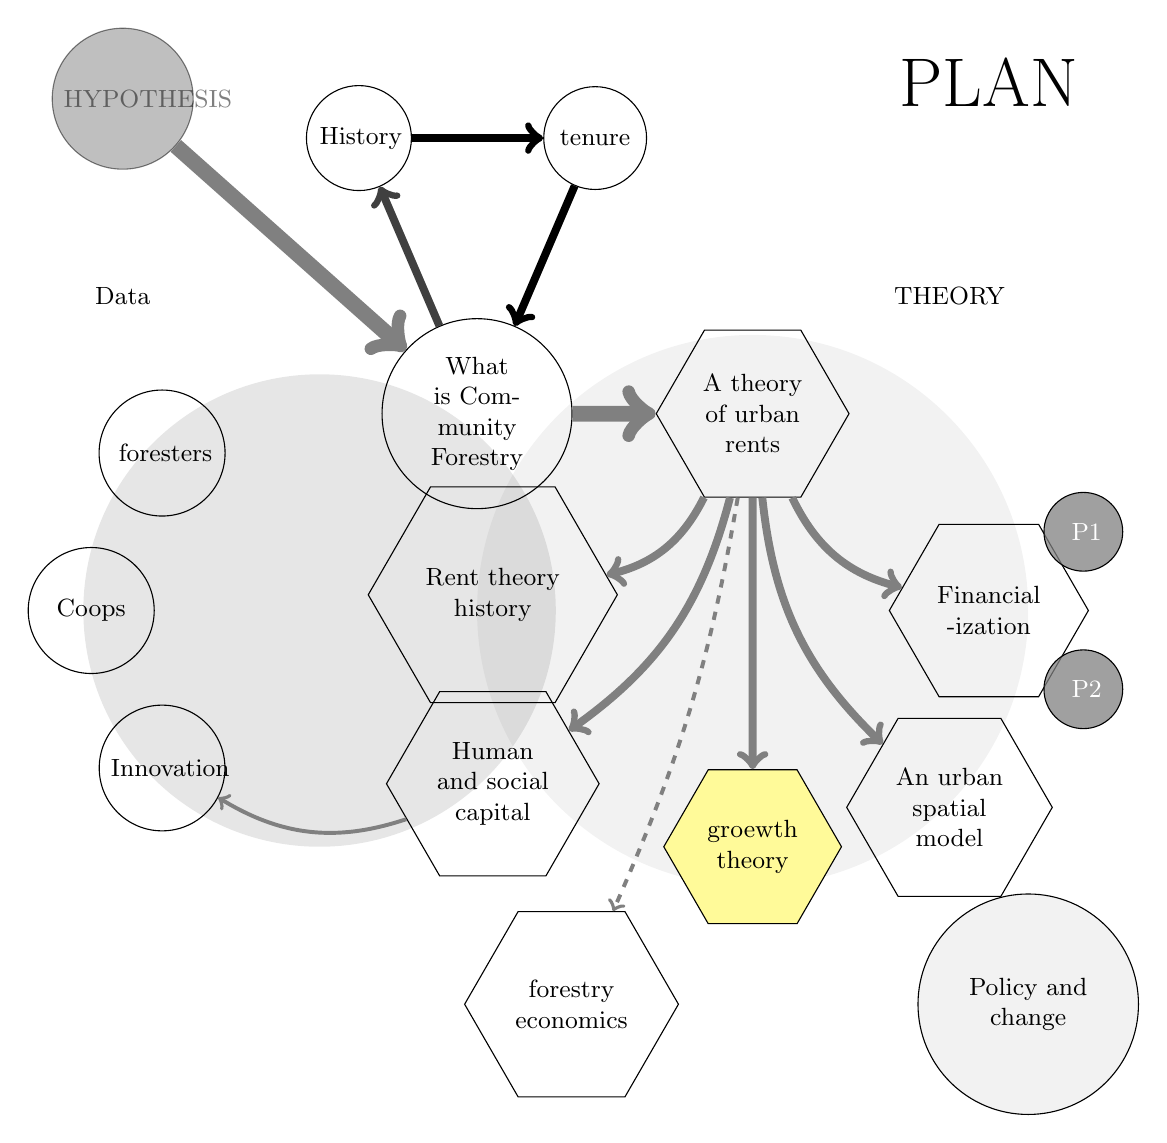
\begin{tikzpicture}%[scale=.8]
    \tikzstyle{every node}=[font=\small]
%\draw[help lines,step=.5] (0,-11) grid (11,11);

%  LOCATION OF ALL NODES
\coordinate (aa) at (-1.5,7.5);%PREFACE
\coordinate (a) at (-1,10);%
 \coordinate (b) at (1.5,7); %history
\coordinate (c) at (6,10); %
\coordinate (d) at (9,9);%
\coordinate (ee) at (-4,7);%
  \coordinate (e) at (-1.5,5); %Community label
\coordinate (f) at (9.5,7.7); %???    PLAN
\coordinate (g) at (9,5); %Economics label
\coordinate (h) at (4.5,7);%tenure
\coordinate (ii) at (-4,4);%
   \coordinate (i) at (1,4);  
\coordinate (j) at (3,3.5);%whatis
\coordinate (k) at (6,4);%
 \coordinate (l) at (6.5,3.5);%joint
\coordinate (mm) at (-1.9,1);%coops
 \coordinate (m) at (1,1);%community grey circle
  \coordinate (n) at (3,1); %
  \coordinate (o) at (9.5,1); %efficiency
				 \coordinate (oo) at (6.5,1);%
				  \coordinate (o1) at (10.7,2);	 \coordinate (o2) at (10.7,0);%Propositions
\coordinate (p) at (9,-1.5);%externalities
				
\coordinate (qq) at (-4,-2);
\coordinate (q) at (-1,-1);%innovation
 \coordinate (r) at (3.2,1.2);%trans
  \coordinate (s) at (3.2,-1.2);%capital
 \coordinate (t) at (6.5,-2);%pubgoods
\coordinate (AA) at (-2,-5);%
 \coordinate (A) at (1,-5);%
\coordinate (B) at (3.7,-4); %
\coordinate (C) at (4.2,-4);%forestryEC
\coordinate (D) at (-1,3);%foresters
\coordinate (EE) at (-1,-8); \coordinate (E) at (1,-8); \coordinate (F) at (3,-8); \coordinate (G) at (6,-8); \coordinate (H) at (10,-4);%Policy
\coordinate (II) at (-4,-11);  \coordinate (I) at (1,-11); \coordinate (J) at (3,-11); \coordinate (K) at (6,-11); \coordinate (L) at (10,-11);
%\coordinate (M) at (coordinate); \coordinate (N) at (coordinate); \coordinate (O) at (coordinate); \coordinate (P) at (coordinate);
%\coordinate (Q) at (coordinate); \coordinate (R) at (coordinate); \coordinate (S) at (coordinate); \coordinate (T) at (coordinate);

%.  CIRCLE NODES
% \fill[red, fill opacity=.8] (0,0) circle (4cm);
\fill [gray, fill opacity=0.2] (m) node [text width=2cm, black, opacity=1] 				(community)	{} circle (3cm);
\fill [gray, fill opacity=0.1] (oo)  node [text width=2cm, align=left, black, opacity=1] 		(econ) {} circle (3.5cm);
\node at (e) [ ] 		(comLtabel) {Data};
\node at (g) [ ] 		(ecLabel) {THEORY};
				%\draw (0,3.2,1) node [text width=1.5cm, text centered] {$Economics$};
			%\draw [fill=red, fill opacity=0.3]  (aa) node [ text width=2cm, black, opacity=1] 									(preface)		{PREFACE: Why, claims} circle (1.4cm);
\node [circle, draw,  fill=gray, opacity=.5,, text width=1.5cm] at			 (aa) 		(preface)		{HYPOTHESIS};
\node [] at			 (f) 		(plan)		{\Huge PLAN};
			%\draw [fill=blue, fill opacity=0.35] (b)node [text width=2cm, align=center, black, opacity=1] 			(history){History: New is Old} circle (1.2cm);
\node[circle, draw, text width=1cm, align=center, black, opacity=1]at 	(b)(history){History} ;
			%\draw [fill=pink, fill opacity=0.5] 		(h) node [text width=2cm, black, opacity=1] 								(tenure) 	{\color{black}tenure} circle (1.2cm);
\node[circle, draw,  text width=1cm, align=center, black] at 				(h) (tenure) 	{tenure} ;
\node[circle, draw,  text width=1.5cm, align=center]at							 (j) (whatis) 	{\color{black}What is Community Forestry} ;
\node[regular polygon, regular polygon sides=6, draw, align=center]at (l) (joint) 	{\color{black}A theory\\ of  urban\\ rents} ;


%\node[circle, draw,  text width=2cm, align=center]at (h) (tenure) 	{\color{black}tenure} ;

%\draw [fill=red, fill opacity=0.5] (j) node [text width=2cm, black, opacity=1] 												(whatis)		{What is Community Forestry}circle (1.4cm);
%\draw [fill=orange, fill opacity=0.5] 	(l) node [text width=2cm, black, text opacity=1] 	               		(joint)	{Joint products}											 circle (1.2cm);
%\draw [fill=green, fill opacity=0] (1,5)node [text width=2cm,red, opacity=1] {Policy and change} circle (1.4cm);
%\draw (q) node [text width=1.3cm, align=center, black, opacity=1] (small)	 {Innovation} circle (1.1cm);
\node[circle, draw,  text width=1.3cm, align=center] at							 (q) (small)	 {Innovation} ;

\draw 	(mm) node [text width=1.3cm, align=center, black, opacity=1] 	(coops) 	{Coops} circle (.8cm);
%\draw [fill=orange, fill opacity=0.5] 	(s) node [text width=2cm,  align=center, black, text opacity=1] (capital) {Human \\and social \\capital} circle (1.2cm);
\node[regular polygon, regular polygon sides=6, draw, align=center] at (s) (capital) {Human \\and social \\capital} ;
%\draw [fill=gray, fill opacity=0.5] 			(o) node [text width=2cm, black, text opacity=1] 						(efficiency)	{Efficiency} circle (1.2cm);
\node[regular polygon, regular polygon sides=6, draw, align=center] at (o) (efficiency)	{Financial\\-ization};
\draw [fill=gray, fill opacity=0.75] (o1) node [text width=.3cm, white, text opacity=1] (	P1)  {P1} 		circle (.5cm);
\draw [fill=gray, fill opacity=0.75] (o2) node [text width=.3cm, white, text opacity=1] (P2) {P2} 			circle (.5cm);

%\draw [fill=orange, fill opacity=0.5] (p) node [text width=2cm, black, opacity=1]					(externalities)	 {externalities} 			circle (1.2cm);
%\draw [fill=orange, fill opacity=0.5] (t)node [text width=2cm, align=center, black, opacity=1] (pubgoods) {public goods} 		circle (1.4cm);
%\draw [fill=orange, fill opacity=0.5] (r) node [text width=2cm, black, opacity=1] 							(trans)	{transaction costs} 		circle (1.1cm);

%.  POLYGON NODES
\node[regular polygon, regular polygon sides=6, draw, align=center] at (p) (externalities)	 {An urban \\spatial\\model};
\node[regular polygon, regular polygon sides=6, draw, align=center, fill=yellow!40] at (t) (pubgoods) {groewth\\theory} ;
\node[regular polygon, regular polygon sides=6, draw, align=center] at (r) (trans)	{Rent theory\\history};



%\draw [fill=yellow, fill opacity=0.15] 	(C) node [text width=2cm, black, opacity=1] 							(forestryEC){forestry \\ economics} circle (1.4cm);
\node[regular polygon, regular polygon sides=6, draw, align=center, fill=gray!.25] at (C) (forestryEC){forestry \\ economics};
\draw [] 	(D) node [text width=1.1cm, black, opacity=1] 							(foresters)	{foresters} circle (.8cm);

  %%%%%JOINT PRODUCTS  AND TRANSACTION COSTS
%\draw [fill=orange, fill opacity=0.5] (G) node [text width=2cm, black, opacity=1] 								{efficiency} circle (1.4cm);
  %%%%%%%%%%%%%%%%%%%%  POLICY CHANGE
\draw [fill=gray, fill opacity=0.1] 		(H)    node [text width=2cm, align=center, opacity=1] 										{Policy and change} circle (1.4cm);

% LINKS
%\draw (J) node [text width=6cm, text centered] {Economic Development };
%\draw ()--();
\draw [gray, line width=2mm,-> ](preface)--(whatis);
\draw  [darkgray, line width=1mm,<- ](history)--(whatis);
\draw  [black, line width=1mm,-> ](tenure)--(whatis);
\draw  [black, line width=1mm,-> ](history)--(tenure);

\draw [gray, line width=2mm,-> ](whatis)--(joint);
\draw [gray, line width=1mm,-> ](joint) to [bend right=25](efficiency);
\draw  [gray, line width=1mm,-> ] (joint) to [bend left=20](capital);
\draw [gray, line width=1mm,-> ](joint) to [bend right=20](externalities);
\draw [gray, line width=1mm,-> ](joint) to [bend left=25](trans);
\draw  [gray, line width=1mm,-> ](joint)->(pubgoods);
\draw  [gray, line width=.5mm,-> ](capital) to[bend left=25](small);
\draw  [gray, line width=.5mm,-> ,dashed](joint) to[bend left=7](forestryEC);
\end{tikzpicture} 

\end{document}